\documentclass{article}
\usepackage[utf8]{inputenc}
\usepackage[document]{ragged2e}
\usepackage{algpseudocode}
\usepackage[]{algorithmicx}
\usepackage{amsmath}
\usepackage{amsthm}
\usepackage{amssymb}
\usepackage[]{listings}
\usepackage{graphicx}
\usepackage{hyperref}
\usepackage{flafter}
\usepackage{subfig}
\usepackage{dsfont}
\graphicspath{ {images/} }

\begin{document}

\begin{titlepage}
	\centering
	
\includegraphics[width=0.15\textwidth]{IIIT-B_logo.jpg}\par\vspace{1cm}
	{\scshape\LARGE International Institute of Information Technology, Bangalore \par}
	\vspace{1cm}
	{\scshape\Large Project Proposal\par}
	{\Large  CS/DS 706 Machine Learning\par}
	\vspace{1.5cm}
	{\huge\bfseries Python Stackoverflow Q\&A Analysis\par}
	\vspace{2cm}
	{\Large\itshape Akanksha Dwivedi - MT2016006\par}
	{\Large\itshape Tarini Chandrashekhar - MT2016144\par}
	\vfill
	Instructor : \par
	Prof. G. Srinivasaraghavan

	\vfill

% Bottom of the page
	{\large \today\par}
\end{titlepage}

\newpage

\tableofcontents

\newpage
\justify

\section{Brief Description}

This project aims at utilising natural language processing and exploratory analytics on a dataset consisting of Python question and answers on Stack Overflow, to design a novel course structure for teaching Python. 

\bigskip
\subsection{Problem Formulation}

\begin{itemize}
\item[$\textendash$] Application/System (Python Course Design)
\begin{itemize}
\item [$\textendash$] MP Module (Exploratory Analytics and Natural Language Processing on Questions and Answers)
\begin{itemize}
\item[$\textendash$] ML task (Unsupervised Text mining)
\begin{itemize}
\item[$\textendash$] Features, Models, Optimization algorithm (to be decided based on empirical observations)
\end{itemize}
\end{itemize}
\end{itemize}
\end{itemize}

\newpage
\section{Dataset}
The dataset consists of full text of questions and answers from StackOverflow, that are tagged with the python tag, useful for natural language processing and community analysis. The dataset is collected over a period of 8 years, from 2008-2016. 
\par
This is organized as three tables i.e three .csv files:

\begin{itemize}
\item \textbf{Questions} contains the title, body, creation date, score, and owner ID for each Python question.

\item \textbf{Answers}  contains the body, creation date, score, and owner ID for each of the answers to these questions. The ParentId column links back to the Questions table.

\item \textbf{Tags} contains the tags on each question besides the Python tag.
\end{itemize}

\newpage

\begin{figure}[h]
\centering
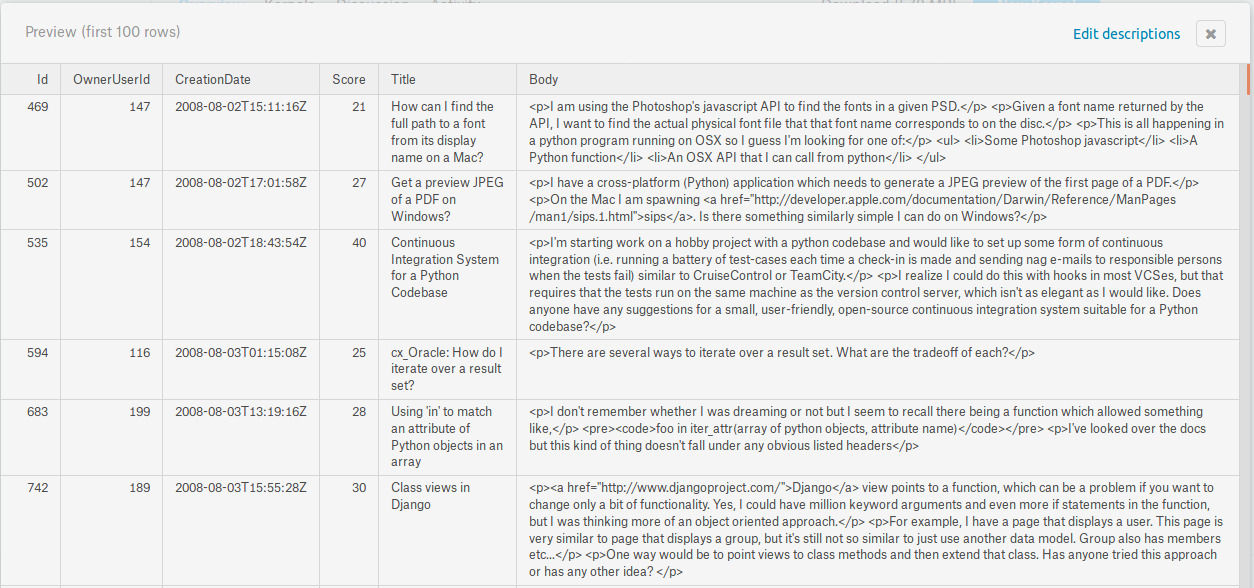
\includegraphics[width=14cm]{Questions}
\caption {Questions.csv}
\end{figure}

\begin{figure}[h]
\centering
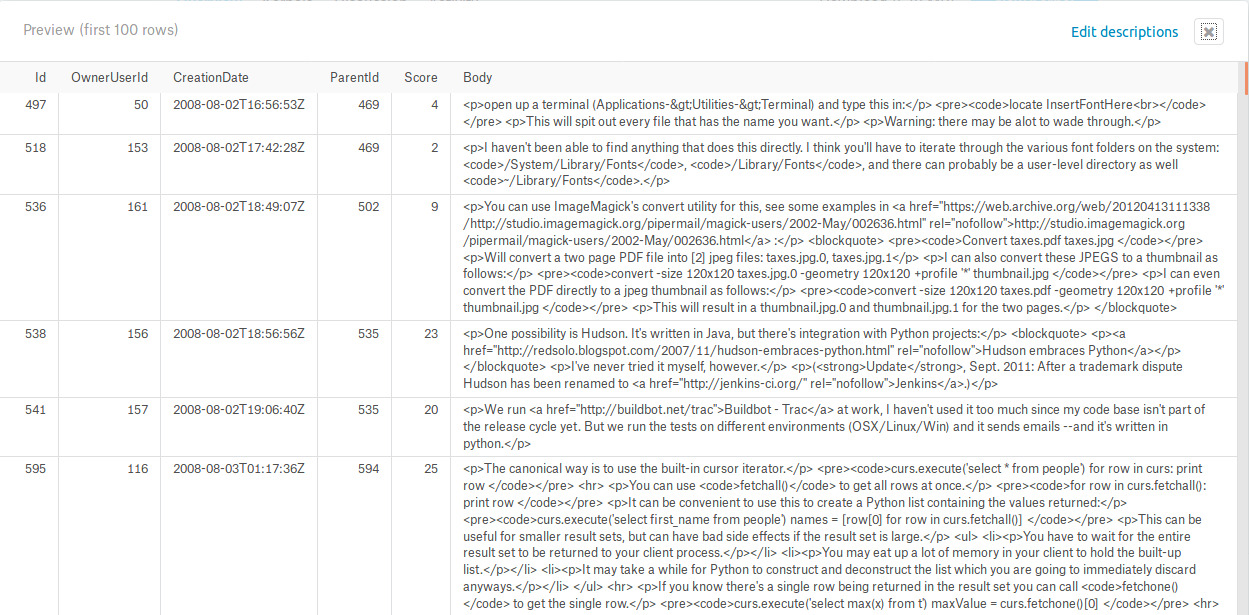
\includegraphics[width=14cm]{Answers}
\caption {Answers.csv}
\end{figure}


\begin{figure}[h]
\centering
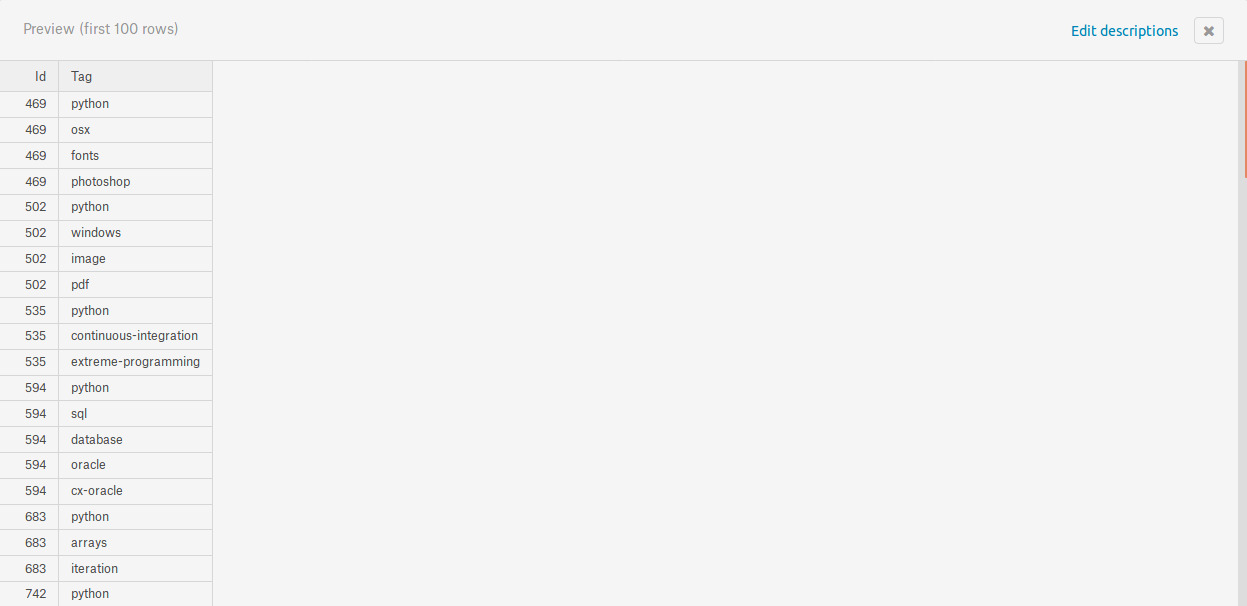
\includegraphics[width=15cm]{Tags}
\caption {Tags.csv}
\end{figure}




\section{Proposed Plan of execution}

\subsection{Milestone 1}
\begin{itemize}
\item Topic association on a rudimentary level by clustering techniques. 
\item Semantic understanding of the dataset.
\end{itemize}

\subsection{Milestone 2}
\begin{itemize}
\item Performing various techniques of Unsupervised Text Analysis on the dataset. 

\item Course structure design based on the filtered dataset, where filtered dataset would be a result of multiple exploratory questions. For example, most asked questions, most discussed questions etc.
\end{itemize}

\subsection{Milestone 3}
\begin{itemize}
\item Augment the course structure designed further to a virtual classroom, with attributes like highest rated users as mentors, most discussed questions as interactive sessions, and so on.

\end{itemize}



\newpage
\section{Main Challenges}
\begin{itemize}
\item The dataset collected is over a long time period, i.e. 8 years, hence relevant data filtering would be a challenge.
\item A very small percentage of questions on Stack Overflow are closed, so we do not have closing timestamp of the questions. So, we cannot explore the lifetime of a question.
\item Judging the merit of a low scoring answer, as genuinely being irrelevant,  being structurally weak or any other inexplicable reason.
\end{itemize} 


\section{Learning Objectives}
\begin{itemize}
\item Experimenting with various unsupervised text mining techniques.
\item Semantic understanding of the text through various Natural Language Processing techniques.
\item Understanding  programming language trends on an active Q\&A platform such as Stack Overflow.
\end{itemize}



\end{document}
